%
% verteilung.tikz -- Verteilungsfunktion für Aufgabe 50000032
%
% (c) 2017 Prof Dr Andreas Müller, Hochschule Rapperswil
%
\documentclass[tikz]{standalone}
\usepackage{times}
\usepackage{txfonts}
\usepackage{pgfplots}
\usepackage{csvsimple}
\usetikzlibrary{arrows,intersections}
\begin{document}
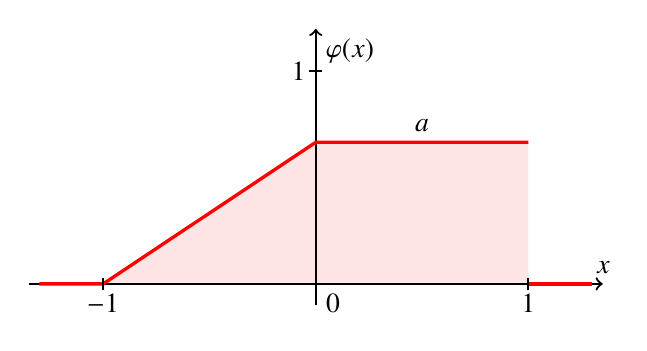
\begin{tikzpicture}[thick,scale=2.7]
\coordinate (O) at (0,0);

\coordinate (A) at (-1,0);
\coordinate (B) at (0,0.666);
\coordinate (C) at (1,0.666);
\coordinate (D) at (1,0);
\coordinate (E) at (0,0);

\coordinate (F) at (-1.3,0);
\coordinate (G) at (1.3,0);

\fill[color=red!10] (A)--(B)--(C)--(D)--(E)--cycle;

\draw[->] (-1.35,0)--(1.35,0) coordinate[label = {above:$x$}];
\draw[->] (0,-0.1)--(0,1.2) coordinate[label={below right:$\varphi(x)$}];

\draw[color=red,line width=1.2] (F)--(A)--(B)--(C);
\draw[color=red,line width=1.2] (D)--(G);

\draw (-1,0.03)--(-1,-0.03);
\draw (1,0.03)--(1,-0.03);
\draw (-0.03,1)--(0.03,1);

\node at (A) [below] {$-1$};
\node at (D) [below] {$1$};
\node at (0,1) [left] {$1$};
\node at (O) [below right] {$0$};
\node at (0.5,0.6666) [above] {$a$};

\end{tikzpicture}
\end{document}
